\documentclass{amsart}
\usepackage[T1]{fontenc}
\usepackage{graphicx}
\usepackage{amsmath}
\usepackage{booktabs}
\usepackage[parfill]{parskip}
\usepackage{cleveref}

\title{Risk and Performance Measurement}
\author{Jakub Kural}
\date{}

\begin{document}

\maketitle{}

Our goal is to study risk and performace of selected stocks from
SP500 index and then try to create an optimal portfolio out of them.
We limit ourselves to companies \emph{KDP, KKR, KIM, KLAC, KMI, KMX, KO,
KEY, KR, KMB} and timeframe from 2022-01-01 to 2025-01-01.

\begin{figure}
  \centering
  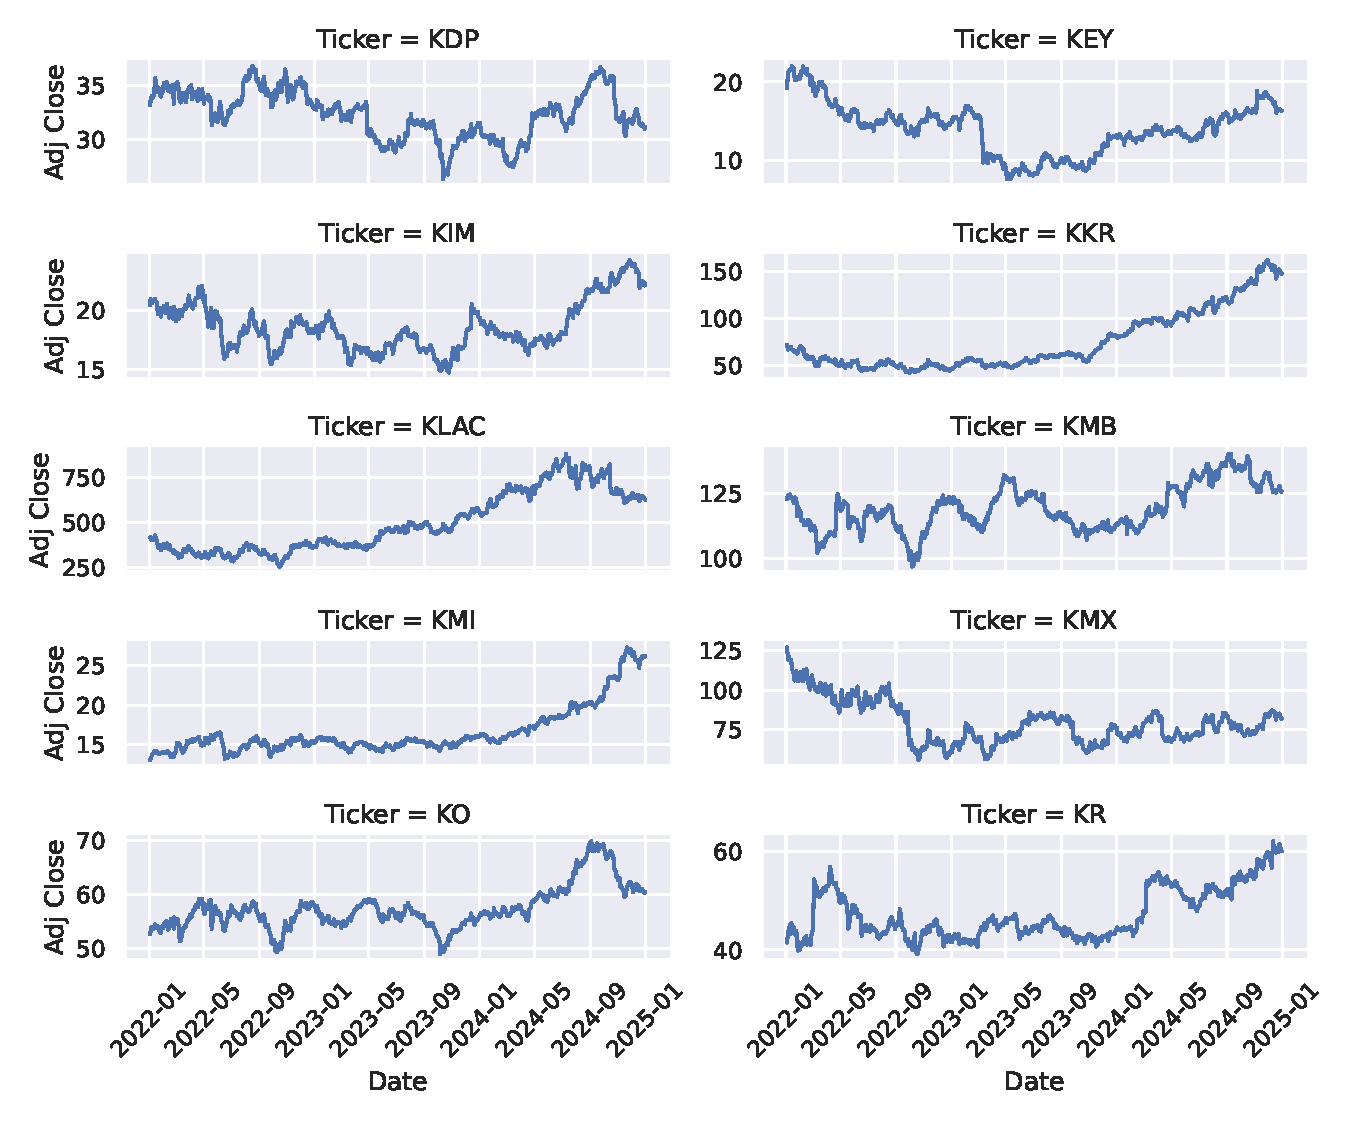
\includegraphics[width=\textwidth]{figs/prices.pdf}
  \caption{Adjusted close prices of the considered stocks}
  \label{fig:prices}
\end{figure}

\section*{General statistical analysis}
We begin by calculating simple returns of the stocks using the formula
\begin{equation}
  R_{i}=\frac{S_{i}-S_{i-1}}{S_{i-1}}
  \label{eq:simple-returns}
\end{equation}
where \(S_i\) is the \(i\)-th observation of the price.


\begin{table}
  \centering
  \input{tables/all_returns_characteristics_1-fixed_pct.tex}
  \begin{tabular}{lrrrrr}
\toprule
Ticker & KMB & KMI & KMX & KO & KR \\
\midrule
count & 752.000000 & 752.000000 & 752.000000 & 752.000000 & 752.000000 \\
mean & 0.000102 & 0.001023 & -0.000213 & 0.000233 & 0.000621 \\
std & 0.011693 & 0.013570 & 0.026994 & 0.009839 & 0.016241 \\
min & -0.057305 & -0.051136 & -0.246008 & -0.069626 & -0.073223 \\
25\% & -0.005995 & -0.006413 & -0.014279 & -0.005277 & -0.007712 \\
50\% & 0.000564 & 0.001012 & -0.000529 & 0.000706 & 0.000444 \\
75\% & 0.006500 & 0.009045 & 0.013998 & 0.005645 & 0.009046 \\
max & 0.081265 & 0.066370 & 0.100741 & 0.038671 & 0.116062 \\
\bottomrule
\end{tabular}

  \caption{Selected statistics of the returns}
  \label{tab:returns-statistics}
\end{table}
\begin{figure}
  \centering
  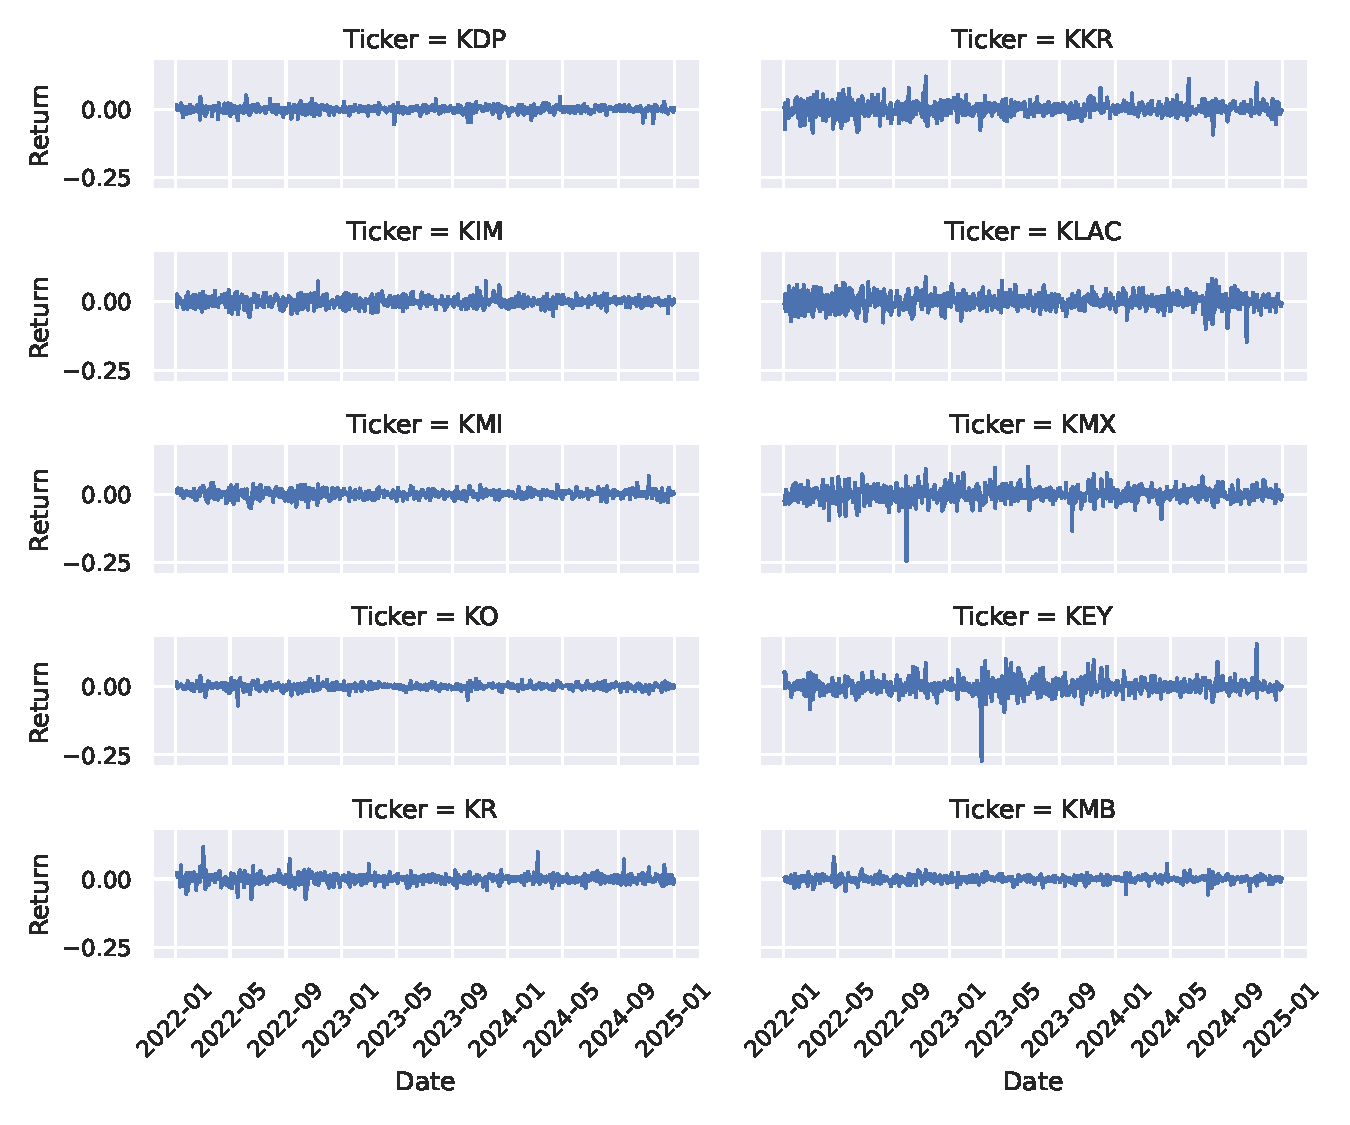
\includegraphics[width=\textwidth]{figs/all_returns.pdf}
  \caption{Returns of the stocks}
  \label{fig:returns}
\end{figure}
\begin{figure}
  \centering
  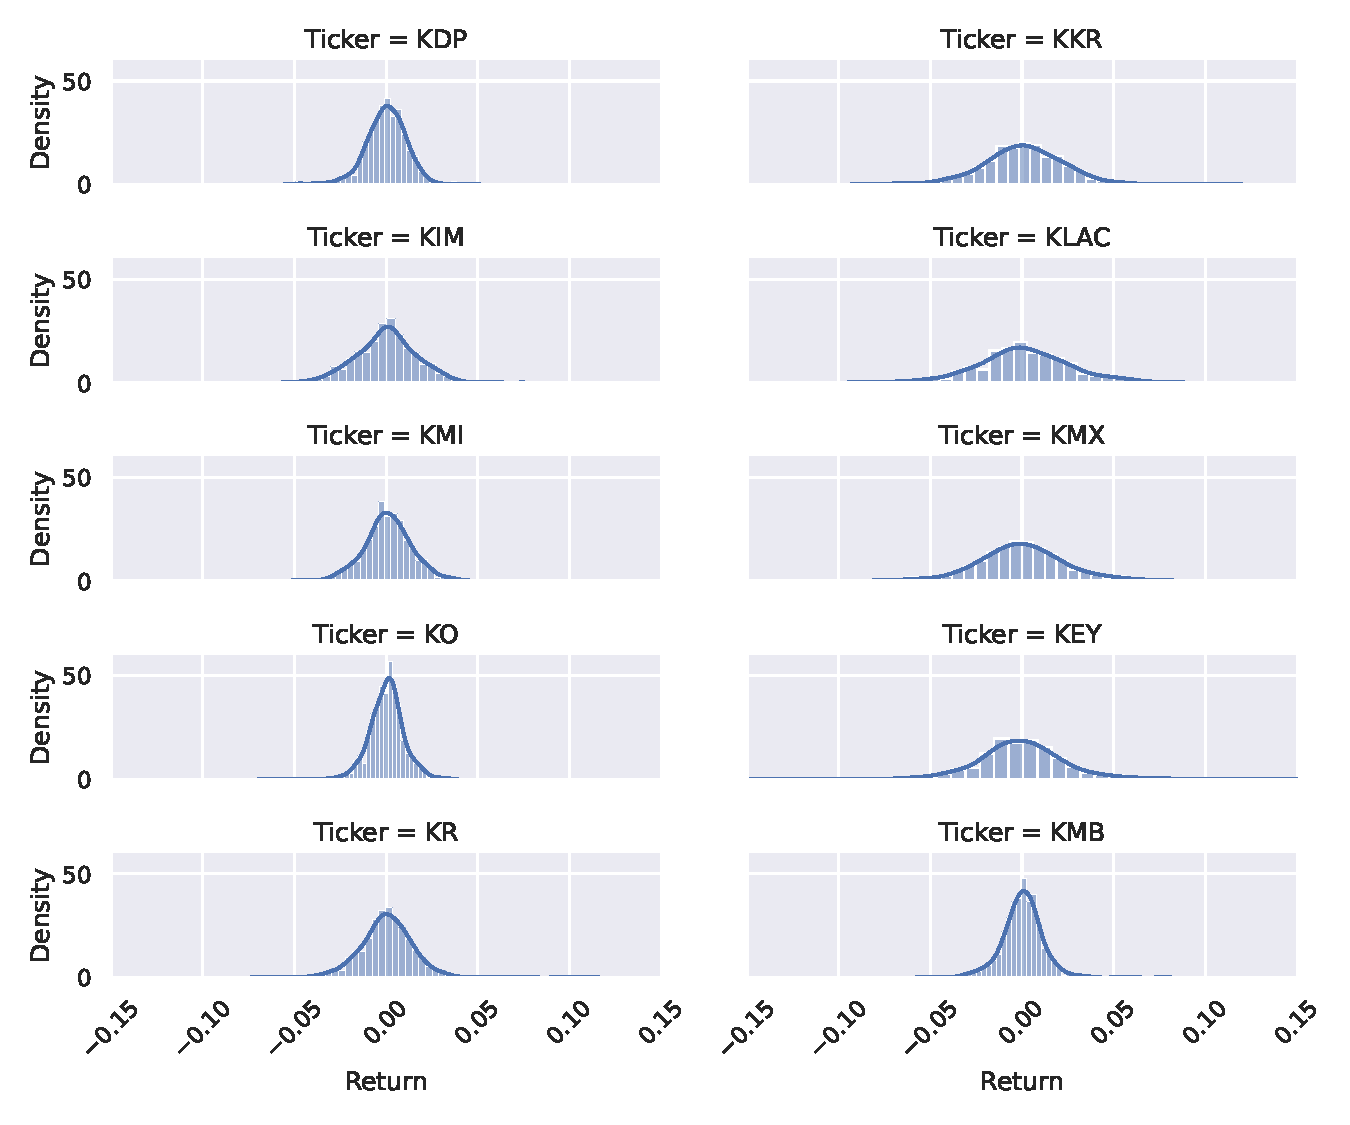
\includegraphics[width=\textwidth]{figs/all_returns_histograms.pdf}
  \caption{Histograms of the returns}
  \label{fig:returns-histograms}
\end{figure}
\begin{figure}
  \centering
  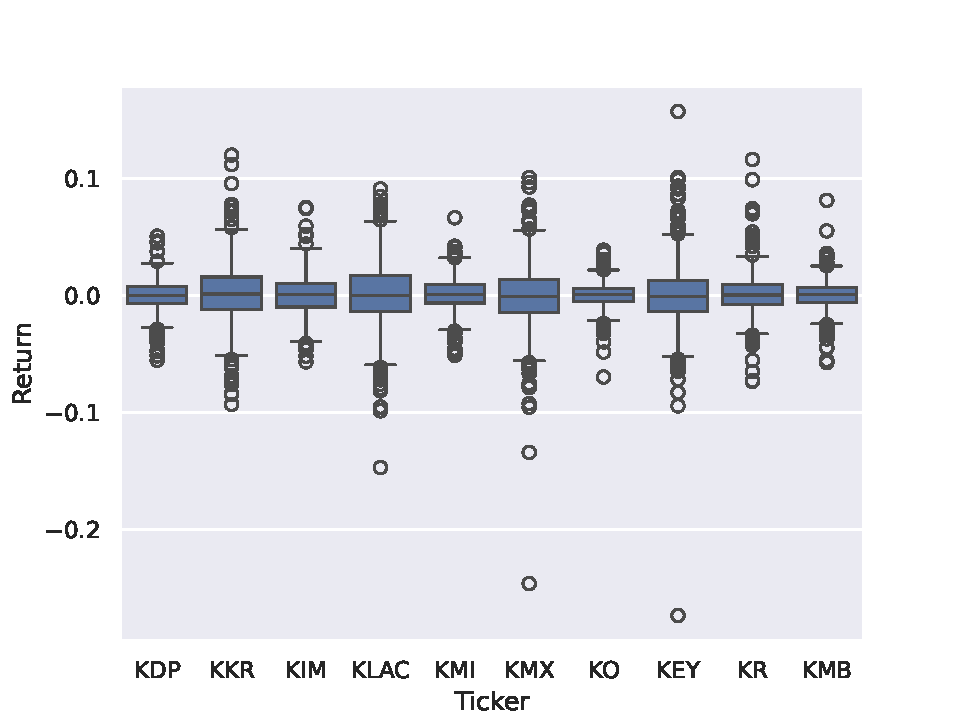
\includegraphics[width=\textwidth]{figs/all_returns_boxplots.pdf}
  \caption{Boxplots of the returns}
  \label{fig:returns-boxplots}
\end{figure}

From tabular data in~\cref{tab:returns-statistics} we can observe that we can
get the highest expected return from stocks \emph{KKR} and \emph{KMI}.
\emph{KMX, KLAC} and \emph{KEY} have the greatest standard deviations.

When viewing histograms~(\cref{fig:returns-histograms}) and
boxplots~(\cref{fig:returns-boxplots}) we can notice that distribution of
the returns for each stock is bell-shaped, however they are tail heavy, as
indicated by the presence of the outliers in boxplots, hinting that the
returns might not be normally distributed.

There are no strong correlations between the returns of individual stocks,
however there are many moderate ones (between \(0.4\) and \(0.6\)), such as
\emph{KO} and \emph{KDP}, \emph{KLAC} and \emph{KKR} and \emph{KO} and
\emph{KMB}. Notably, \emph{KR} and \emph{KLAC} are the least correlated at
correlation coefficient equal to \(0.034\)~(\cref{fig:returns-correlation})

\begin{figure}
  \centering
  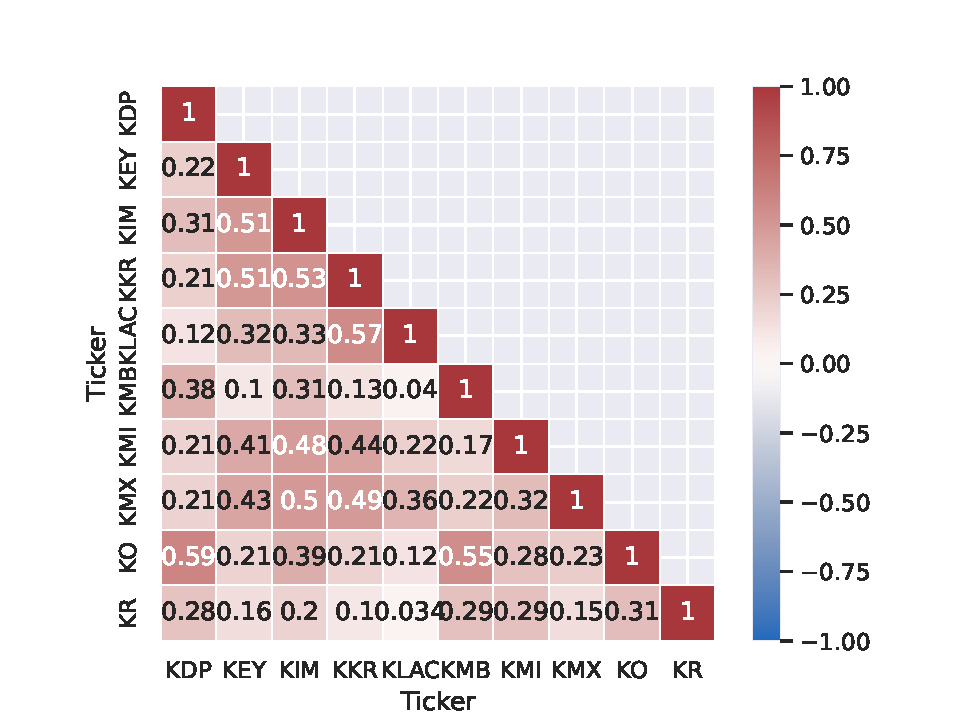
\includegraphics[width=\textwidth]{figs/all_returns_correlation.pdf}
  \caption{Correlation matrix of returns}
  \label{fig:returns-correlation}
\end{figure}

\section*{Risk and performance analysis}

Now we proceed to measure the risk and performance of the stocks. We begin
with a fund of \$2000 that we invest in the stocks individually. Since we are
investing into stocks directly (and not, for example, their derivatives) and
we assume no impact of time on the price, value of the portolio is simply
the sum of the price of each stock multiplied by their amount in the portfolio.
Therefore, we can calculate the P\&L simply by scaling (and averaging in the
case of multiple risk factors) the returns, as shown in the following
derivation:
\begin{equation}
  \begin{split}
    \text{P\&L}_{i} &= P(S^{1}_{i}, \ldots, S^{k}_{i-1}) - P(S^{1}_{i-1}, \ldots, S^{k}_{i-1})\\
                    &= \sum_{j=1}^{k} a^{j}_{i} \left(S^{j}_{i} - S^{j}_{i-1}\right)\\
                    &= \sum_{j=1}^{k} a^{j}_{i} S^{j}_{i-1} \frac{S^{j}_{i}-S^{j}_{i-1}}{S^{j}_{i-1}}\\
                    &= V_{i}\sum_{j=1}^{k} w^{j}_{i} R^{j}_{i}
  \end{split}
  \label{eq:scaling-of-portfolio}
\end{equation}
where \(a^{j}_{i}\) is the amount of stock \(j\) in the portfolio at time \(i\),
\(V_{i}=\sum_{j=1}^{k} a^{j}_{i} S^{j}_{i}\) is the total value of the portfolio
at time \(i\) and \(w^{j}_{i}=\frac{a^{j}_{i} S^{j}_{i}}{V_{i}}\) is the weight
of the stock \(j\) in the portfolio at time \(i\).

We measure expected value, standard deviation, value at risk, expected shortfall,
Sharpe Ratio and Gain Loss Ratio for the P\&Ls. Mean provides information about
expected daily gain from the investment, standard deviation provides information
about how far we can expected realized return from the mean. Value at risk and
expected shortall provide information about how much money is necessary to protect
the invested capital from going into negative. We also choose Sharpe Ratio
and Gain Loss Ratio to measure performance of the investment. Sharpe Ratio
is a simple performance measurement that considers the average gain from a
portfolio and divides it by its volatility (standard deviation). Gain Loss Ratio
is similar to Sharpe Ratio, however it only punishes losses instead of general
volatility and it is also monotone.

\begin{table}
  \centering
  \begin{tabular}{lrrrrr}
\toprule
Ticker & KDP & KEY & KIM & KKR & KLAC \\
\midrule
mean & 0.111549 & -1.612251 & -0.518326 & -2.660523 & -0.096134 \\
std & 26.701978 & 44.740059 & 38.679135 & 60.940105 & 61.633868 \\
VaR 1\% & 73.803531 & 106.918129 & 91.817132 & 158.588664 & 143.473237 \\
ES 2.5\% & 69.980046 & 107.528323 & 90.282911 & 150.180229 & 132.200728 \\
SR & 0.004178 & -0.036036 & -0.013401 & -0.043658 & -0.001560 \\
GLR & 0.005100 & 0.000000 & 0.000000 & 0.000000 & 0.000000 \\
\bottomrule
\end{tabular}

  \begin{tabular}{lrrrrr}
\toprule
Ticker & KMB & KMI & KMX & KO & KR \\
\midrule
mean & 0.089794 & 1.592800 & -4.767310 & 0.949275 & 0.485229 \\
std & 27.666452 & 34.391119 & 65.107958 & 24.846839 & 42.065761 \\
VaR 1\% & 71.431328 & 95.653861 & 174.067389 & 72.100231 & 137.662384 \\
ES 2.5\% & 67.721324 & 89.683336 & 209.756450 & 71.995370 & 114.439372 \\
SR & 0.003246 & 0.046314 & -0.073222 & 0.038205 & 0.011535 \\
GLR & 0.004353 & 0.058961 & 0.000000 & 0.048219 & 0.016835 \\
\bottomrule
\end{tabular}

  \caption{Performance of \$2000 in each stock}
  \label{tab:pnl-2000-each}
\end{table}

From~\cref{tab:pnl-2000-each} we can see that \emph{KEY, KIM, KKR, KLAC, KMX}
on average lose money and have high variance. This implies that they probably
are not a good investment. Stocks with the gratest Sharpe Ratios are \emph{KMI,
KD} and \emph{KO}. Incidentally, they also have the greatest Gain Loss Ratios.
Based on that they seem to be the best investments from the considered stocks.

We also consider a portfolio optimized in the following way: for risk aversion
coefficients \(\gamma \in [-0.05, 0]\) we find the weights for which the
mean-variance criterion is maximized. It can be interpreted that for a given
mean we find weights of the portfolio that minimaze the variance, and therefore
risk.

\begin{figure}
  \centering
  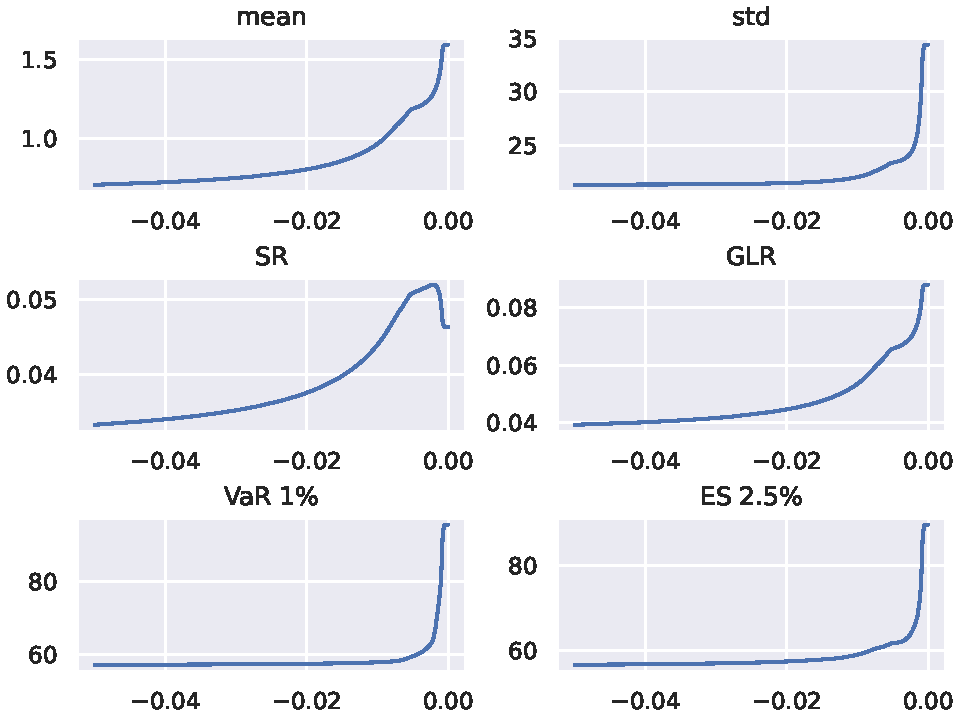
\includegraphics[width=\textwidth]{figs/frontier_stats.pdf}
  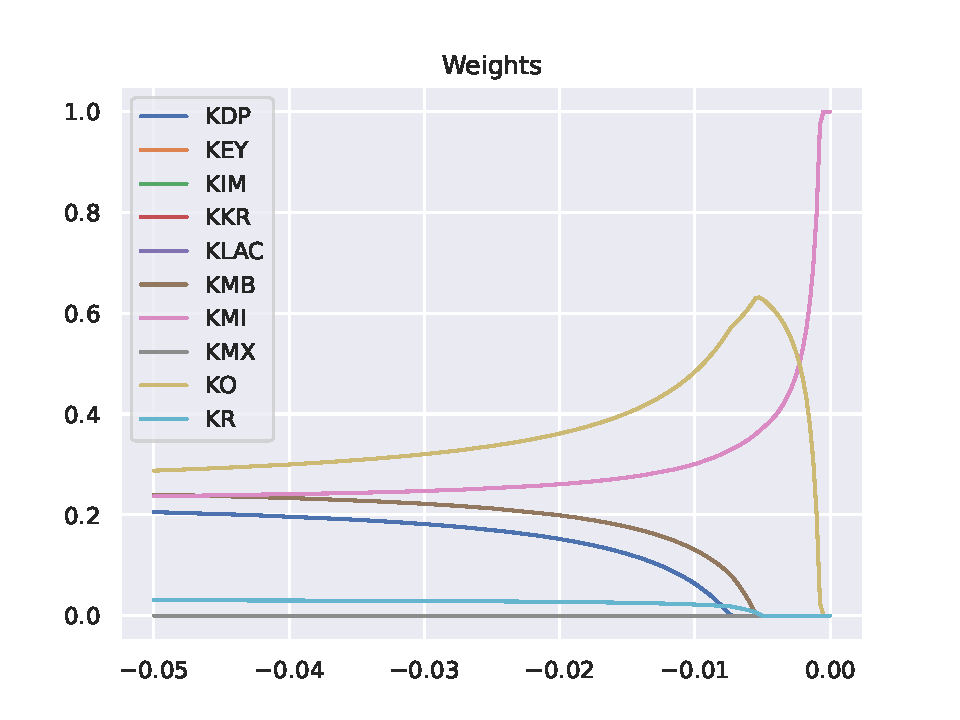
\includegraphics[width=\textwidth]{figs/frontier_weights.pdf}
  \caption{Statistics and weights for different values of \(\gamma\)}
  \label{fig:frontier}
\end{figure}

We can see that, as the risk tolerance increases, all statistics rise
and weights become less diversified. For the optimum portfolio we choose
portfolio which maximizes Sharpe Ratio, which rougly corresponds to
\(\gamma = -0.002\).

\begin{figure}
  \centering
  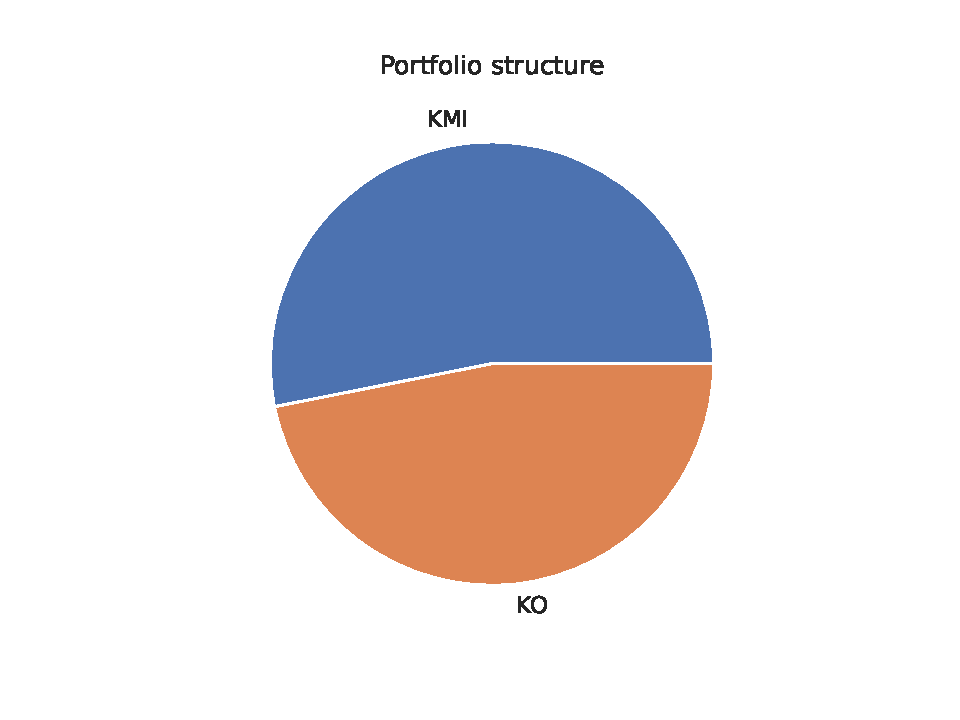
\includegraphics[width=\textwidth]{figs/portfolio_structure.pdf}
  \caption{Structure of optimal portfolio. It contains only 2 stocks}
  \label{fig:structure}
\end{figure}

\begin{table}
  \centering
  \begin{tabular}{lrrrr}
\toprule
 & Chosen & Other & All & Optimized \\
\midrule
mean & 0.884541 & -1.297075 & -0.642590 & 1.291076 \\
std & 22.426515 & 35.170556 & 29.687338 & 24.861026 \\
VaR 1\% & 58.018137 & 97.583469 & 79.200238 & 64.934100 \\
ES 2.5\% & 56.840641 & 90.297836 & 77.390130 & 65.397958 \\
SR & 0.039442 & -0.036880 & -0.021645 & 0.051932 \\
GLR & 0.048367 & 0.000000 & 0.000000 & 0.065753 \\
\bottomrule
\end{tabular}

  \caption{Performance of mixed portfolios of \$2000}
  \label{tab:pnl-mixed}
\end{table}

From tables \cref{tab:pnl-2000-each} and \cref{tab:pnl-mixed} we can see
that the optimized portfolio has greater Sharpe Ratio and Gain Loss Ratio
than any individual stock. Portfolio of best individual stocks with equal
weights has lower performace than the best individual stock, but at much
lower volatility, VaR and ES. Portfolio of other stocks and all stocks
don't perform well, but they have relatively small standard deviations.
Diversification has greatly reduced standard deviation, and in the case of
the optimized portfolio, has increased performance of individual stocks.

In my opinion, the best investment is the optimized portolio, because
it only has slightly greater variance, VaR and ES than the mix of the 3 best
performing portfolios, while having much greater mean, SR and GLR.

\section*{Backtesting}
In order to test our hypotheses, we perform a VaR backtest on our portfolios.
As the consequence of~\cref{eq:scaling-of-portfolio}, we only need to backtest
the returns.

\begin{figure}
  \centering
  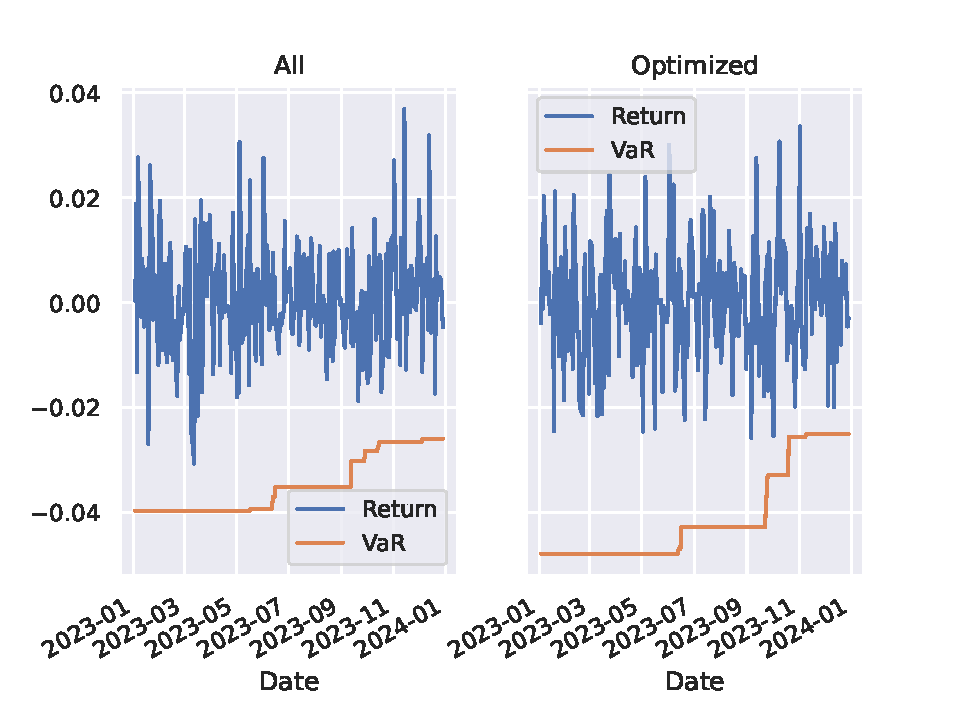
\includegraphics[width=\textwidth]{figs/var_backtest.pdf}
  \caption{The results of the VaR backtest on the portfolios}
  \label{fig:var-backtest}
\end{figure}

As we can see in~\cref{fig:var-backtest}, we have experienced no exceptions,
meaning that our predictions have successfully protected our portfolios.
However, this doesn't mean that our prediction correctly models price movement.
In order to measure that, we perform PIT backtest, that is, check if the empirical
distribution of the returns correctly model realized returns.

\begin{figure}
  \centering
  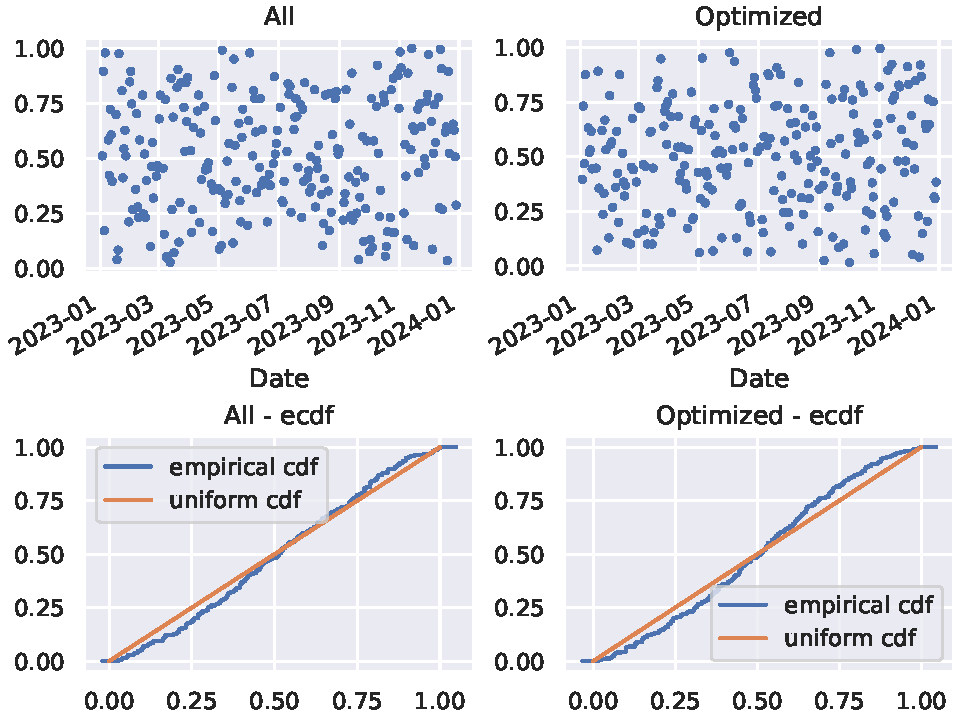
\includegraphics[width=\textwidth]{figs/pit_backtest.pdf}
  \caption{The results of the PIT backtest on the portfolios}
  \label{fig:pit-backtest}
\end{figure}

Visual inspection of~\cref{fig:pit-backtest} suggests that both average portfolio
and optimized portfolio pass the backtest, as the resulting distribution is
close to uniform. It is further confirmed by the Kolmogorov-Smirnov test,
as the results from~\cref{tab:pit-gof} can't refute the hypothesis, that the
distribution is uniform.

\begin{table}
  \centering
  \begin{tabular}{lrr}
    \toprule
    Portfolio & statistic & p value\\
    \midrule
    All       &     0.076 &     0.1\\
    Optimized &     0.076 &     0.1\\
    \bottomrule
  \end{tabular}
  \caption{Results of PIT portfolio goodness of fit test to uniform distribution}
  \label{tab:pit-gof}
\end{table}

The performance of the portfolios in 2024 is presented in~\cref{tab:pnl-2024}.
We can see that the optimal portfolio still has greater mean, SR and GLR than
portfolio of all stocks. However, its std, VaR and ES are also greater.
Because of that, for an investor with higher tolerance for risk, the optimized
portfolio seems like a better investment. There is a moderate correlation
between the portfolios, as the correlation coefficient is equal to 0.57.

\begin{table}
  \centering
  \begin{tabular}{lrr}
\toprule
 & All & Optimized \\
\midrule
mean & 1.950528 & 4.087038 \\
std & 16.695499 & 23.444081 \\
VaR 1\% & 46.097739 & 58.313855 \\
ES 2.5\% & 41.987442 & 52.764781 \\
SR & 0.116830 & 0.174331 \\
GLR & 0.163592 & 0.280288 \\
\bottomrule
\end{tabular}

  \caption{Performance of portfolios in 2024-2025}
  \label{tab:pnl-2024}
\end{table}

\end{document}
